\subsubsection{Continuum models}

	Continuum models of the motion of several liquids in a porous medium are widespread and useful, among them are Darcy's Law, Buckley-Leverett, etc. 

	\subsubsection{Relative phase permeability}
	
	\subsubsection{Capillary pressure.
A feature of these classical models is that the relative phase permeability and capillary pressure are considered a function of saturation
This is true as long as the characteristic time of the processes is much longer than the characteristic time of fluid redistribution in the capillary space.
In some cases, this assumption is incorrect.
For example, when the saturation changes rapidly, or when the porous medium has such a structure that the time of fluid redistribution is long (fractured-porous medium with blocks and cracks)

2. There are a number of continuum models that take these effects into account. Among them, we note the articles by Hasanizade, Barenblatt and Kondaurov. The first two take into account not only saturation, but also the rate of saturation change.
The Kondaurov model, along with saturation, considers a special nonequilibrium parameter, which should relax to an equilibrium value.

3. In order to better understand the models of nonequilibrium filtration (fluid movement), it is necessary to simulate fluid movement at the micro level (that is, at the scale of individual pores and capillaries)
There are a number of approaches to such modeling. Example: or a direct Navier-Stokes calculation.
In addition, network models are used. They are simpler.
We list models from the literature, advantages and disadvantages.

4. We decided to go the way of network models and create our own network model.
The following is a detailed description of our model.
It is necessary to describe the geometry of the capillaries, the rules for overcoming nodes (here is the novelty of the work!).
Give the calculation algorithm. Describe a numerical method.

5. Next, give the problem statements and results. Don't skimp on pictures and graphs!
We need to start with the pressure drop.
Finish with impregnation and saturation relaxation.




\subsection{The Problem}
	Figure \ref{fig_capillary_flow_brick} is an example of two-phase flow in porous body. The wetting fluid, in this case - water displaces the non wetting fluid - air. The aim is to plot concentration of one of the phases with respect to time for a given region of the porous body, similar to \cite{fatt1956network}. In this work, we focus on the process of wetting fluid entering the region of finer pores, in our model denoted by thinner radius.
	
	\begin{figure}[H]
		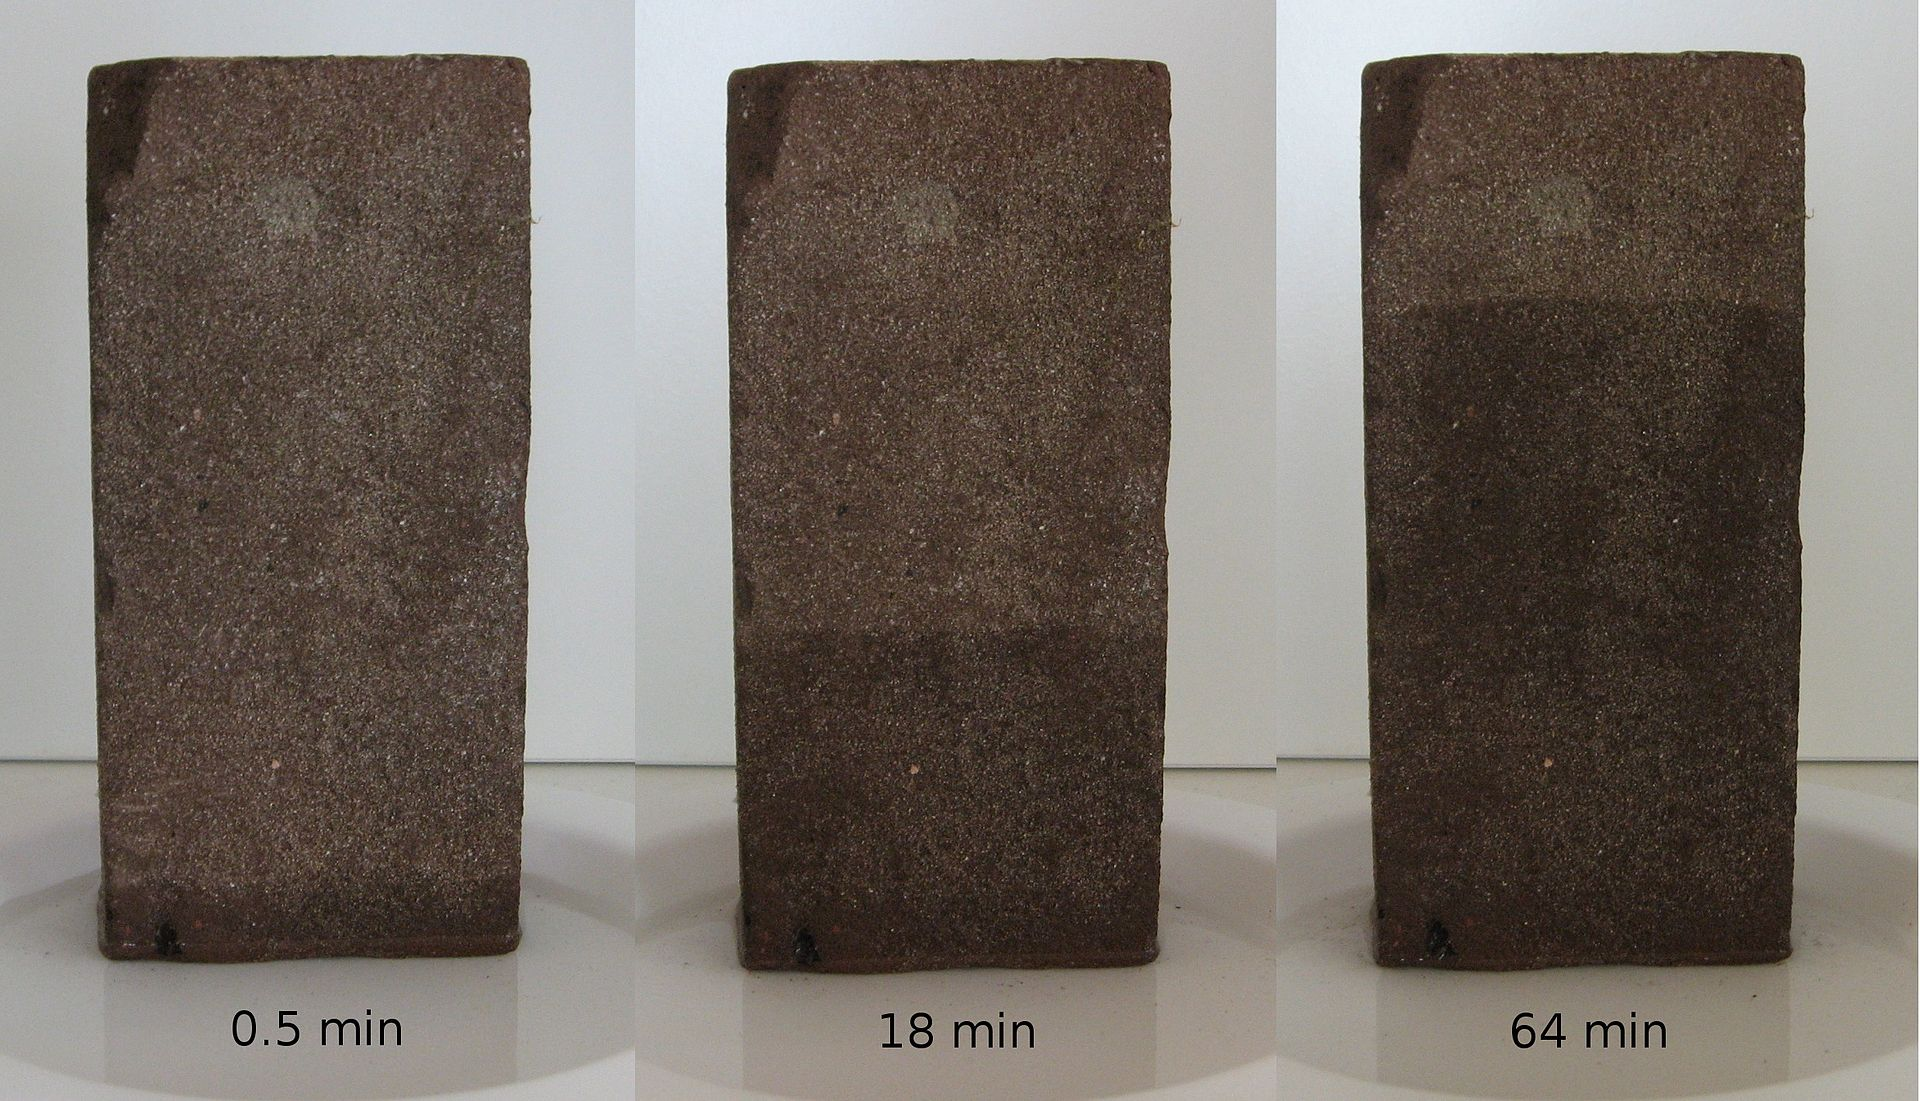
\includegraphics[height=8cm]{fig_capillary_flow_brick}
		\caption{Water climbing against gravity through a porous medium. \cite{wiki:Capillary_action}}
		\label{fig_capillary_flow_brick}
	\end{figure}
	
\subsection{About Other Models}
	Besides network models, various other models have been developed. For example in \cite{fatt1956network}, the flow was simulated by using a network of resistors. In our model, variation of radius across tubes exists, while they have varied the resistance of the resistors. However in this case it is difficult to model the capillary pressure drop. In \cite{aker1998two}, the simulation was conducted using hour glass shaped model of tubes, where the average flow rate is given by the Washburn equation for capillary flow \cite{washburn1921dynamics}, the disadvantage is that the must be approximated to be cylindrical even tough the capillary pressure varies as its position in the tube. 
	
	
	Regarding the applications of modeling two phase flow in water-oil displacements, non-equilibrium effects were considered by \cite{barenblatt2003mathematical}, where it is concluded that the non-equilibrium effects should be taken into account. Other network models include, such as \cite{chen1985pore} and \cite{king1987fractal}, however these models did not demonstrate the displacement of the wetting fluid into the region with thinner radius or channels. The processing of optimizing the process generating relation between nodes is similar to that in \cite{raoof2010new}. 
		
\subsection{Continuum Scale Models}
	\subsubsection{Darcy's Law}
		Darcy's law is a fundamental equation in fluid mechanics that describes the flow of fluids through porous media. It was formulated by Henry Darcy in 1856 and has since become a vary important part of hydro geology, petroleum engineering, and other fields dealing with fluid flow in porous media.
		Darcy's law states that the flow rate Q of a fluid through a porous medium is directly proportional to the pressure gradient $(\Delta P)$ and the cross-sectional area A of the medium, and inversely proportional to the length L of the medium. Mathematically, it can be expressed as:

		\[ Q = - k \cdot A \cdot \frac{\Delta P}{L} \]

		\begin{itemize}
			\item $Q$ is the volumetric flow rate of the fluid (m$^3$/s).
			
			\item $k$ is the permeability of the porous medium (m$^2$).
			
			\item $A$ is the cross-sectional area perpendicular to the flow direction (m$^2$).
			
			\item $\Delta P$ is the pressure difference along the flow direction (Pa).
			
			\item $L$ is the length of the porous medium in the flow direction (m).
			
		\end{itemize}
	
		Darcy's law is widely used in the modeling and analysis of two-phase flow in porous media. Two-phase flow refers to the simultaneous flow of two immiscible fluids, such as gas and liquid, through a porous medium. In this context, Darcy's law can be extended to account for the flow of both phases.
		
		One common application of Darcy's law in two-phase flow modeling is in the field of petroleum engineering, specifically in reservoir engineering. When modeling the flow of oil and gas in an underground reservoir, Darcy's law is used to estimate the flow rates and pressure distributions within the reservoir. By considering the relative permeability of oil and gas, the equation can be modified to account for the presence of two phases and their interactions \cite{uhlmann2005immersed}.
		
		Additionally, Darcy's law is often combined with other equations, such as the continuity equation and material balance equations, to create more comprehensive models for two-phase flow. These models can help predict the behavior of fluid flows in porous media, optimize production strategies, and estimate recovery factors in oil and gas reservoirs.
	
	\subsubsection{Buckley-Everett Theory}
		The Buckley-Leverett theory, also known as the fractional flow theory, is a mathematical model that describes the displacement of one fluid by another in porous media. It is widely used in the field of petroleum engineering 
		
		The Buckley-Leverett equation describes the fractional flow of one fluid phase (often called the displacing phase) as a function of the saturation of the other fluid phase (often called the displaced phase). Mathematically, the equation is given as:
		
		The equation is given by:
	
		\[ f = \frac{{(S_w - S_{wc})}}{{(1 - S_{wc} - S_{or})}} \]
		
		where:
		\begin{itemize}
			\item \( f \) is the fractional flow of the displacing phase.
			
			\item \( S_w \) is the saturation of the displaced phase (a fractional value between 0 and 1).
			
			\item \( S_{wc} \) is the critical water saturation (the saturation at which the capillary pressure becomes zero).
			
			\item \( S_{or} \) is the residual oil saturation (the saturation of oil that remains trapped in the rock after water flooding).
			
		\end{itemize}
	
		The Buckley-Leverett theory assumes that the fluids involved are incompressible and that the flow is governed by Darcy's law. The theory provides a framework to study the displacement of one fluid by another and predict the behaviour of the fluid fronts as they move through the porous medium.
		The key assumption in the Buckley-Leverett theory is that the fluids are flowing as distinct phases and that they exhibit capillary pressure and relative permeability characteristics. Capillary pressure represents the pressure difference between the two fluids at the fluid-fluid interface, and relative permeability describes the fractional flow of each fluid phase as a function of its saturation.

\subsection{Empirical Models}
	\subsubsection{Corey and Brooks- Corey models}
		The Corey-Brooks Corey model, also known as the Corey-Brooks model or the Corey-Brooks-Kohoutek model, is an extension of the Buckley-Leverett theory.
	
		The Corey-Brooks Corey model introduces an empirical function to describe the relative permeability curves for the two phases (typically water and oil) as a function of their respective saturation. The model assumes that the relative permeabilities are influenced by capillary pressure and can be expressed using power law relationships.
		
		The relative permeability curves for the displaced (wetting) phase (typically water) and the displacing (non-wetting) phase (typically oil) are defined as follows:

		The equations are given by:

		\[ k_{ro} = k_{ro_{\text{max}}} \cdot (1 - S_w - S_{ro})^n \]
		\[ k_{rw} = k_{rw_{\text{max}}} \cdot S_w^m \]
		 
		where:
		\begin{itemize}
			\item  \( k_{ro} \) is the relative permeability of the non-wetting phase (oil).
			
			\item\( k_{rw} \) is the relative permeability of the wetting phase (water).
			
			\item \( k_{ro_{\text{max}}} \) and \( k_{rw_{\text{max}}} \) are the maximum relative permeabilities of the non-wetting and wetting phases, respectively.
			
			\item \( S_w \) is the water saturation (a fractional value between 0 and 1).
			
			\item \( S_{ro} \) is the residual oil saturation (the saturation of oil that remains trapped in the rock after water flooding).
			
			\item \( n \) and \( m \) are empirical exponents that govern the shape of the relative permeability curves.
			
		\end{itemize}

		The Corey-Brooks Corey model allows for the estimation of relative permeability curves for the wetting and non-wetting phases based on laboratory measurements or historical data. These curves are crucial in characterizing the flow behavior and predicting fluid displacement in porous media.
		
		By incorporating the relative permeability curves into the Buckley-Leverett equation, the Corey-Brooks Corey model enables the simulation and prediction of two-phase flow behavior, such as fluid front movement and displacement efficiency, in reservoirs or aquifers. This information is valuable for optimizing production strategies, designing water flooding operations, and assessing the potential for enhanced oil recovery techniques \cite{tryggvason2001front}.

	\subsubsection{ Leverett-J-function}
		The Leverett-J function, also known as the Leverett function or the J function, is a mathematical expression used in two-phase flow modeling to describe the capillary pressure-saturation relationship in porous media. It is an extension of the Buckley-Leverett theory. 

		The Leverett-J function relates the capillary pressure (Pc) to the saturation (Sw) of the wetting phase (usually water). The function describes how the capillary pressure changes with the saturation, providing insights into the fluid-fluid interactions and flow characteristics in the porous medium.
		
		The Leverett-J function is expressed as follows:

		\[ J = \frac{{\frac{{dS_w}}{{dP_c}}}}{{\frac{{S_w}}{{P_c}}}} \]

		where:
		\begin{itemize}
			\item 	 \( J \) is the Leverett-J function.
			
			\item \( S_w \) is the saturation of the wetting phase (a fractional value between 0 and 1).
			
			\item \( P_c \) is the capillary pressure.
			
		\end{itemize}

		The Leverett-J function is used in two-phase flow modeling to estimate various parameters and analyze fluid displacement behavior. Some applications of the Leverett-J function include:
		
		\begin{enumerate}
			\item Estimating relative permeabilities
			
			\item Predicting fluid displacement
			
			\item Assessing reservoir connectivity
			
			\item Optimizing enhanced oil recovery (EOR) techniques, it helps in understanding the capillary pressure distribution and identifying areas of bypassed oil
			
		\end{enumerate}
		
\subsection{Pore-Scale Methods}
	\subsubsection{Lattice Boltzmann Method (LBM)}
		The Lattice Boltzmann Method (LBM) is a computational fluid dynamics (CFD) technique used to simulate fluid flow and solve complex fluid dynamics problems. It is particularly useful for modeling two-phase flow, where two immiscible fluids flow through a domain with interfacial interactions.
		
		Unlike traditional CFD methods based on solving the Navier-Stokes equations, the Lattice Boltzmann Method operates on a mesoscopic scale and simulates fluid flow by modeling the behavior of particles (often referred to as "lattice cells") on a discrete lattice. It uses a kinetic approach to solve the Boltzmann equation, which describes the evolution of particle distribution functions \cite{aidun2010lattice}.
		
		The Lattice Boltzmann Method is advantageous for modeling two-phase flow because it naturally captures interfacial phenomena, such as fluid-fluid interfaces, droplet dynamics, and interfacial tension effects. It can handle complex geometries and is capable of capturing mesoscale phenomena like droplet coalescence, breakup, and multiphase interactions \cite{yudistiawan2009higher}.
	
		The application of LBM in two-phase flow modeling involves the following steps:
		
		\begin{enumerate}
			\item Lattice Construction: The computational domain is discretized into a lattice structure.
			
			\item Particle Distribution: These distribution functions evolve based on collision and streaming processes.
			
			\item Collision and Streaming: The distribution functions undergo a collision step, where particles interact and exchange momentum and energy. After the collision, the particles stream to neighboring lattice cells based on predefined velocity directions.
			
			\item Macroscopic Properties: Macroscopic fluid properties such as density, velocity, and pressure are calculated from the distribution functions.
			
			\item Interfacial Effects: Interfacial phenomena, such as surface tension and interfacial forces, are incorporated into the Lattice Boltzmann Method.
			
		\end{enumerate}
		
	\subsubsection{Direct Numerical Simulation NAVIER-STOKES}
	
		Direct Numerical Simulation (DNS) is a computational technique used to solve the complete set of equations governing fluid flow without any turbulence modeling assumptions. It provides a detailed and accurate representation of fluid behavior by discretizing the governing equations in space and time and solving them numerically. DNS is particularly useful for studying turbulent flows, where turbulence models often introduce uncertainties and limitations.

		By performing DNS of two-phase flow, researchers can gain insights into various phenomena and phenomena of interest, such as bubble or droplet breakup, coalescence, collision dynamics, and heat and mass transfer between the phases. DNS can also be used to investigate complex multiphase flows, such as bubbly flows, particle-laden flows, or flows with phase change \cite{chen1998lattice}.
		
		The application of DNS in modeling two-phase flow offers several advantages:
		
		\begin{enumerate}
			\item Accuracy: DNS provides a high level of accuracy and resolves small-scale turbulent structures.
			
			\item Detailed information: DNS captures detailed information about the flow, such as velocity profiles, vorticity, and pressure distribution.
			
			\item Validation of models: DNS can be used to validate and improve existing turbulence models.
			
			\item Design optimization: DNS helps in optimizing the design of various systems involving two-phase flows, such as heat exchangers, chemical reactors, and combustion chambers.
			
			\item Fundamental understanding: DNS aids in developing a fundamental understanding of the underlying physics of two-phase flow.
			
		\end{enumerate}
			 
\subsection{Hybrid and Upscalling Approaches}
	\subsubsection{Hybrid Models}
		A hybrid model, in the context of two-phase flow modeling, refers to a combination of different modeling approaches or techniques to capture the complexities and improve the accuracy of simulations. It involves integrating multiple models or methods, each designed to address specific aspects of the flow behavior, to create a more comprehensive and accurate representation of the system \cite{rabbani2018pore}.

		Here are a few examples of hybrid modeling approaches commonly used:
		
		\begin{enumerate}
			\item Coupling of Continuum and Discrete Models: This approach combines continuum-based models, such as the finite element method (FEM) or finite difference method (FDM), with discrete models, such as lattice Boltzmann method (LBM) or pore network models. Continuum models are used to capture the overall behavior of the flow field, while discrete models focus on capturing specific phenomena at a smaller scale, such as interfacial dynamics or fluid-fluid interactions. The coupling allows for a more accurate representation of complex flow behavior.
			
			\item Multiphase Flow with Computational Fluid Dynamics (CFD) and Volume-of-Fluid (VOF) Method: In this approach, CFD methods are used to solve the Navier-Stokes equations and simulate the fluid flow, while the Volume-of-Fluid method is employed to track the fluid interface and capture the two-phase flow behavior. CFD provides detailed information on velocity and pressure fields, while VOF method accurately captures the shape and movement of the fluid interface.
			
			\item Combination of Empirical and Mechanistic Models: Hybrid models can combine empirical correlations, such as relative permeability or capillary pressure models, with mechanistic models that describe fluid behavior based on fundamental principles, such as the Buckley-Leverett theory or Darcy's law. This allows for a more accurate representation of flow behavior by incorporating both empirical knowledge and physics-based understanding.
		\end{enumerate}
		
		The specific formulas used in hybrid models depend on the combination of models and methods being employed. 

		The choice of the hybrid modeling approach and the formulas used depends on the specific objectives, computational resources available, and the level of accuracy required in capturing the two-phase flow behavior \cite{tropea2007springer}.

	\subsubsection{Upscalling Techniques}
	
		Upscaling techniques in two-phase flow modeling refer to methods that aim to represent the behavior of fluid flow at a larger scale, such as the reservoir scale, based on information obtained at a smaller scale, such as the pore scale. These techniques are employed to reduce the computational cost and improve the efficiency of simulating two-phase flow in large-scale reservoirs or heterogeneous porous media \cite{gong2021dynamic}, \cite{valvatne2004predictive}.

		The application of upscaling techniques in two-phase flow modeling involves the following steps:

		\begin{enumerate}
			\item Characterization of Heterogeneous Media:	The porous media are characterized at a fine scale, typically using methods such as core analysis, well logs. This provides information on the spatial distribution of rock and fluid properties, such as porosity, permeability, and saturation, at a small scale.

			\item Selection of Upscaling Approach:	Various upscaling techniques can be employed based on the nature of the porous media and the properties of interest. Some common upscaling approaches include arithmetic averaging, geometric averaging, and flow-based upscaling methods such as the streamline-based or multiscale finite volume methods.

			\item Upscaling Equations:	The upscaling technique involves deriving equations or relationships that connect the fine-scale properties to the coarse-scale properties. These equations capture the effective behavior of the flow variables, such as effective permeability or relative permeability, at the larger scale.

			\item Coarse-Grid Simulation: Using the upscaled properties and equations, a simulation is performed at the coarse scale. This involves solving the governing equations, such as Darcy's law or the continuity equation, on a coarser grid that represents the larger-scale domain.
			
		\end{enumerate}
		
		Some common formulas used in upscaling techniques for two-phase flow modeling include:

		\begin{enumerate}
		
			\item Effective Permeability: The effective permeability at the coarse scale is often computed using an averaging technique, such as arithmetic or geometric averaging, applied to the fine-scale permeability values. For example, arithmetic averaging is given by:
			
			The equation is given by:

			\[ K_{\text{eff}} = \frac{1}{V} \int K \, dV \]

			where:
			\begin{itemize}
				\item   \( K_{\text{eff}} \) is the effective permeability.
				
				\item \( K \) is the fine-scale permeability.
				
				\item  \( V \) is the volume of the representative elementary volume (REV) at the coarse scale.
				
			\end{itemize}


			\item Relative Permeability: The relative permeability at the coarse scale is derived based on the relative permeability curves obtained at the fine scale. Different upscaling approaches, such as the Brooks-Corey model or the Corey-Brooks Corey model, can be employed to obtain the effective relative permeability curves at the coarse scale.

			\item Capillary Pressure: Upscaling capillary pressure involves relating the fine-scale capillary pressure-saturation relationship to the coarse-scale properties. Various methods, such as the Leverett-J function or a pore network-based approach, can be used to upscale the capillary pressure.
		
		\end{enumerate}

		Upscaling techniques are essential for simulating large-scale two-phase flow systems, such as reservoirs, efficiently and accurately. They allow for the transfer of information from small-scale simulations to larger scales, thereby reducing computational costs while preserving the key flow behavior and properties. The choice of upscaling technique depends on the characteristics of the porous media and the desired level of accuracy in the simulation\cite{pope2000turbulent}.
